\section{Farmaci del sistema respiratorio}

\subsection{Asma}

\begin{tikzpicture}
	\tikzset{level 2/.style={level distance=130pt}}
	\tikzset{level 3/.style={level distance=130pt}}
	\Tree
	[.Asma
		[.{malattia infiammatoria\\ delle vie aeree}
			{infiammazione}
			[.{ostruzione bronchiale}
				{solitamente reversibile}
				{in alcuni casi irreversibile}
			]
			{iperreattività agli allergeni}
		]
	]	
\end{tikzpicture}

\begin{tikzpicture}
	\Tree
	[.sintomi
		{sibili respiratori}
		{dispnea}
		tosse
		{costrizione torace}
	]
\end{tikzpicture}

\begin{tikzpicture}
	\tikzset{level distance=80pt}
	\Tree
	[.fisiopatogenesi
		[.{ingesso allergene}
			[.{APC presentano\\ antigeni ai \ce{T_H_2}}
				[.{\ce{T_H_2} stimolano B\\ a produrre IgE}
					[.{IgE si legano\\ agli allergeni}
						\node[dummyc]{};
					]
				]
			]
		]
	]
	\begin{scope}[yshift=-6em]
	\Tree
	[.\node[dummyc]{};
		[.{Mastociti legano IgE}
			{fase immediata}
			{fase tardiva}
		]
	]
	\end{scope}
\end{tikzpicture}

\begin{tikzpicture}
	\tikzset{level 1/.style={level distance=75pt}}
	\tikzset{level 2/.style={level distance=90pt}}
	\tikzset{level 3/.style={level distance=90pt}}
	\tikzset{level 4/.style={level distance=80pt}}
	\Tree
	[.{fase immediata}
		[.{mastociti\\ liberano}
			[.istamina
				[.{liberazione \ce{Ca^2+} nel REL}
					{broncospasmo}
				]
			]
			[.{leucotreni/citochina}
				[.IL5
					[.{attivazione eosinofili}
						{danno tissutale}
						{edema}
						{congestione}
					]
					[.{fase tardiva}
					]
				]
				[.IL4
					{stimolo a produrre IgE}
				]
			]
			[.{fattori di crescita}
			]
		]
	]
\end{tikzpicture}

\begin{tikzpicture}
	\tikzset{level distance=140pt}
	\Tree
	[.{fase tardiva}
		{inspessimento della parete\\ con restringimento del lume}
		{flogosi}
		rimodellamento
		{$\uparrow$produzione muco}
	]
\end{tikzpicture}

tutto ciò causa iperresponsività bronchiale futura.

\begin{tikzpicture}
	\tikzset{level distance=140pt}
	\Tree
	[.{farmaci}
		[.{broncodilatatori\\ (a breve durata d'azione)}
		]
		[.{glucocorticosteroidi\\ (in aerosol)}
		]
		[.{broncodilatatori\\(a lunga durata d'azione)}
		]
		[.{metilxantine o\\ antagonisti dei leucotreni}
		]
		[.{corticosteroidi orali}
		]
		[.{anticorpi monoclonali anti--IgE}
		]
	]
	\begin{scope}[xshift=18em]
		\draw[drawarrow] (0,2) -> (0,-2);
		\node[text width=8em] at (2,0){step operativi via via che la malattia diventa più grave};
	\end{scope}
\end{tikzpicture}



\newpage